%!TeX root=../tempestrackham.tex

\Act*{2}
\Scene*{1}[Another part of the island.]

\begin{figure}[t]
	\centering
	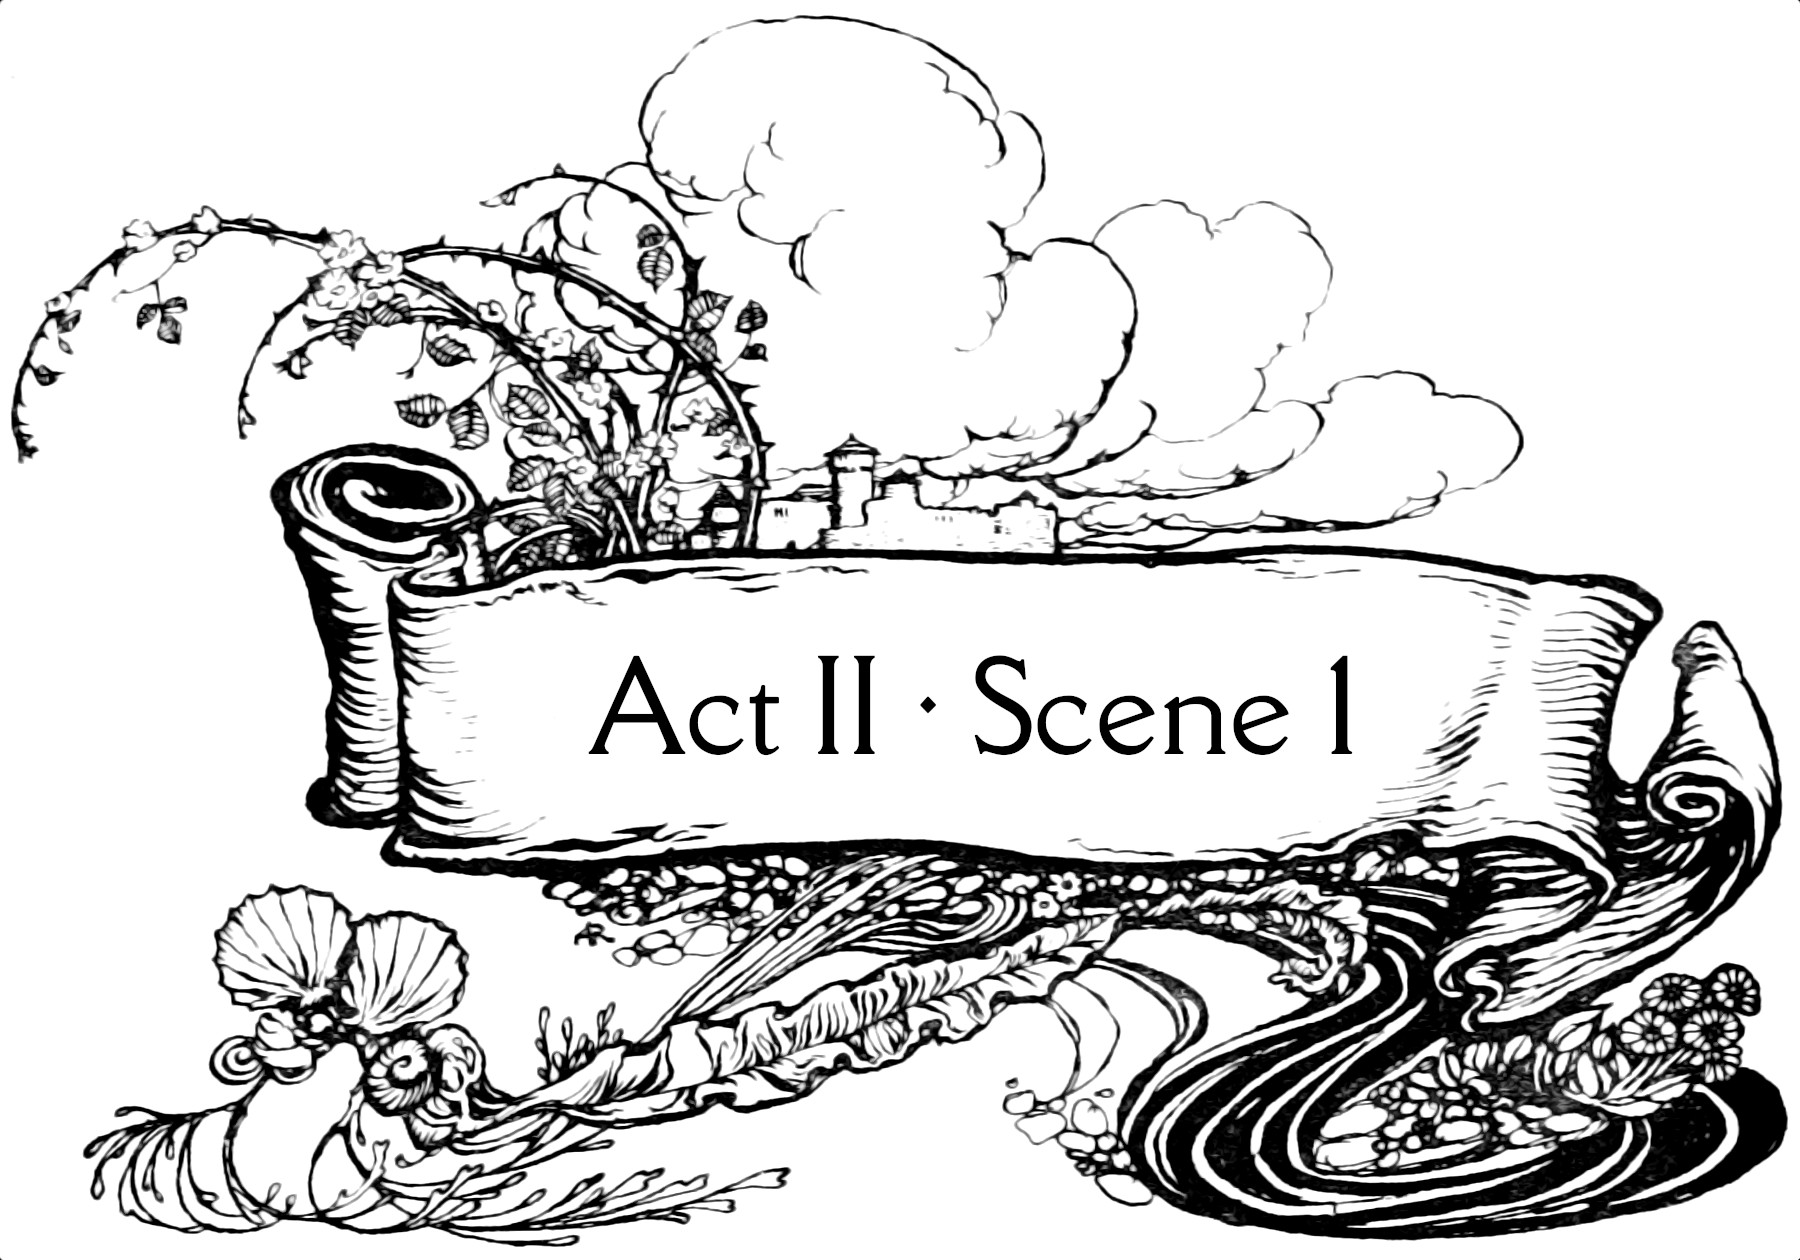
\includegraphics[width=\headerwidth]{2ihead}
\end{figure}


\vspace{\textsink}
\textit{(Another part of the island.)}\centering

\enter{\textsc{Alonso}, \textsc{Sebastian}, \textsc{Antonio}, \textsc{Gonzalo}, \textsc{Adrian}, \textsc{Francisco}, and others}

\begin{verse_speech}[Gonzalo] 
\textit{(To \textsc{Alonso})} 
Beseech you, sir, be merry; you have cause,\\
So have we all, of joy; for our escape\\
Is much beyond our loss. Our hint of woe\\
Is common; every day some sailor's wife,\\
The masters of some merchant and the merchant\\
Have just our theme of woe; but for the miracle,\\
I mean our preservation, few in millions\\
Can speak like us: then wisely, good sir, weigh\\
Our sorrow with our comfort.
\end{verse_speech}

\verseline[Alonso]{Prithee, peace.} 
\verseline[Sebastian]{\asideto{Antonio}{He receives comfort like cold porridge.}}
\verseline[Antonio]{The visitor will not give him o'er so.} 
\begin{prose_speech}[Sebastian] Look he's winding up the watch of his wit; by and by it will strike.
\end{prose_speech}

\verseline[Gonzalo]{\textit{(To \textsc{Alonso})} Sir,—} 
\verseline[Sebastian]{One: tell.} 
\begin{verse_speech}[Gonzalo] When every grief is entertain'd that's offer'd,\\
Comes to the entertainer—
\end{verse_speech}

\verseline[Sebastian]{A dollar.} 
\begin{prose_speech}[Gonzalo] Dolour comes to him, indeed: you have spoken truer than you purposed.
\end{prose_speech}

\verseline[Sebastian]{You have taken it wiselier than I meant you should.} 
\verseline[Gonzalo]{\textit{(To \textsc{Alonso})} 
Therefore, my lord,—} 
\verseline[Antonio]{Fie, what a spendthrift is he of his tongue!} 
\verseline[Alonso]{\textit{(To \textsc{Gonzalo})} 
I prithee, spare.} 
\verseline[Gonzalo]{Well, I have done: but yet,—} 
\verseline[Sebastian]{\asideto{Antonio}{He will be talking.} }
\begin{prose_speech}[Antonio] 
\asideto{Sebastian}{Which, of he or Adrian, for a good wager, first begins to crow?}
\end{prose_speech}

\verseline[Sebastian]{The old cock.} 
\verseline[Antonio]{The cockerel.} 
\verseline[Sebastian]{Done. The wager?} 
\verseline[Antonio]{A laughter.} 
\verseline[Sebastian]{A match!} 
\verseline[Adrian]{Though this island seem to be desert,—} 
\verseline[Sebastian]{Ha, ha, ha! So, you're paid.} 
\verseline[Adrian]{Uninhabitable and almost inaccessible,—} 
\verseline[Sebastian]{Yet,—} 
\verseline[Adrian]{Yet,—} 
\verseline[Antonio]{He could not miss't.} 
\verseline[Adrian]{It must needs be of subtle, tender and delicate temperance.}
\verseline[Antonio]{Temperance was a delicate wench.} 
\verseline[Sebastian]{Ay, and a subtle; as he most learnedly delivered.} 
\verseline[Adrian]{The air breathes upon us here most sweetly.} 
\verseline[Sebastian]{As if it had lungs and rotten ones.} 
\verseline[Antonio]{Or as 'twere perfumed by a fen.} 
\verseline[Gonzalo]{Here is everything advantageous to life.} 
\verseline[Antonio]{True; save means to live.} 
\verseline[Sebastian]{Of that there's none, or little.} 
\verseline[Gonzalo]{How lush and lusty the grass looks! how green!} 
\verseline[Antonio]{The ground indeed is tawny.} 
\verseline[Sebastian]{With an eye of green in't.} 
\verseline[Antonio]{He misses not much.} 
\verseline[Sebastian]{No; he doth but mistake the truth totally.} 
\verseline[Gonzalo]{But the rarity of it is,—which is indeed almost} 
beyond credit,—
\verseline[Sebastian]{As many vouched rarities are.} 
\begin{prose_speech}[Gonzalo] That our garments, being, as they were, drenched in the sea, hold notwithstanding their freshness and glosses, being rather new-dyed than stained with salt water.
\end{prose_speech}

\verseline[Antonio]{If but one of his pockets could speak, would it not say he lies?}
\verseline[Sebastian]{Ay, or very falsely pocket up his report} 
\begin{prose_speech}[Gonzalo] Methinks our garments are now as fresh as when we put them on first in Afric, at the marriage of the king's fair daughter Claribel to the King of Tunis.
\end{prose_speech}

\verseline[Sebastian]{'Twas a sweet marriage, and we prosper well in our return.} 
\verseline[Adrian]{Tunis was never graced before with such a paragon to} 
their queen.
\verseline[Gonzalo]{Not since widow Dido's time.} 
\verseline[Antonio]{Widow! a pox o' that! How came that widow in? widow Dido!}
\verseline[Sebastian]{What if he had said <widower Æneas> too? Good Lord,
how you take it!}
\verseline[Adrian]{\textit{(To \textsc{Gonzalo})} <Widow Dido> said you? you make me study of that: she was of Carthage, not of Tunis.}
\verseline[Gonzalo]{This Tunis, sir, was Carthage.} 
\verseline[Adrian]{Carthage?} 
\verseline[Gonzalo]{I assure you, Carthage.} 
\verseline[Sebastian]{His word is more than the miraculous harp; he hath} 
raised the wall and houses too.
\verseline[Antonio]{What impossible matter will he make easy next?} 
\verseline[Sebastian]{I think he will carry this island home in his pocket} 
and give it his son for an apple.
\verseline[Antonio]{And, sowing the kernels of it in the sea, bring} 
forth more islands.
\verseline[Gonzalo]{Ay.} 
\verseline[Antonio]{Why, in good time.} 
\verseline[Gonzalo]{\textit{(To \textsc{Alonso})} Sir, we were talking that our garments seem now} 
as fresh as when we were at Tunis at the marriage
of your daughter, who is now queen.
\verseline[Antonio]{And the rarest that e'er came there.} 
\verseline[Sebastian]{Bate, I beseech you, widow Dido.} 
\verseline[Antonio]{O, widow Dido! ay, widow Dido.} 
\verseline[Gonzalo]{\textit{(To \textsc{Alonso})} Is not, sir, my doublet as fresh as the first day I wore it? I mean, in a sort.}
\verseline[Antonio]{That sort was well fished for.} 
\verseline[Gonzalo]{\textit{(To \textsc{Alonso})} When I wore it at your daughter's marriage?} 
\begin{verse_speech}[Alonso] 
You cram these words into mine ears against\\
The stomach of my sense. Would I had never\\
Married my daughter there! for, coming thence,\\
My son is lost and, in my rate, she too,\\
Who is so far from Italy removed\\
I ne'er again shall see her. O thou mine heir\\
Of Naples and of Milan, what strange fish\\
Hath made his meal on thee?
\end{verse_speech}

\begin{verse_speech}[Francisco] 
Sir, he may live:\\
I saw him beat the surges under him,\\
And ride upon their backs; he trod the water,\\
Whose enmity he flung aside, and breasted\\
The surge most swoln that met him; his bold head\\
'Bove the contentious waves he kept, and oar'd\\
Himself with his good arms in lusty stroke\\
To the shore, that o'er his wave-worn basis bow'd,\\
As stooping to relieve him: I not doubt\\
He came alive to land.
\end{verse_speech}

\verseline[Alonso]{No, no, he's gone.} 
\begin{verse_speech}[Sebastian] 
Sir, you may thank yourself for this great loss,\\
That would not bless our Europe with your daughter,\\
But rather lose her to an African;\\
Where she at least is banish'd from your eye,\\
Who hath cause to wet the grief on't.
\end{verse_speech}

\verseline[Alonso]{Prithee, peace.} 
\begin{verse_speech}[Sebastian] 
You were kneel'd to and importuned otherwise\\
By all of us, and the fair soul herself\\
Weigh'd between loathness and obedience, at\\
Which end o' the beam should bow. We have lost your son,\\
I fear, for ever: Milan and Naples have\\
More widows in them of this business' making\\
Than we bring men to comfort them:\\
The fault's your own.
\end{verse_speech}

\verseline[Alonso]{So is the dear'st o' the loss.} 
\begin{verse_speech}[Gonzalo] My lord Sebastian,\\
The truth you speak doth lack some gentleness\\
And time to speak it in: you rub the sore,\\
When you should bring the plaster.
\end{verse_speech}

\verseline[Sebastian]{Very well.} 
\verseline[Antonio]{And most chirurgeonly.} 
\begin{verse_speech}[Gonzalo] 
\textit{(To \textsc{Alonso})} It is foul weather in us all, good sir, \\
When you are cloudy.
\end{verse_speech}

\verseline[Sebastian]{\hspace{\widthof{When you are cloudy.}}Foul weather?} 
\verseline[Antonio]{\hspace{\widthof{When you are cloudy. Foul weather?}}Very foul.} 
\verseline[Gonzalo]{Had I plantation of this isle, my lord,—} 
\verseline[Antonio]{He'ld sow't with nettle-seed.} 
\verseline[Sebastian]{Or docks, or mallows.} 
\verseline[Gonzalo]{And were the king on't, what would I do?} 
\verseline[Sebastian]{'Scape being drunk for want of wine.} 
\begin{verse_speech}[Gonzalo] 
I' the commonwealth I would by contraries\\
Execute all things; for no kind of traffic\\
Would I admit; no name of magistrate;\\
Letters should not be known; riches, poverty,\\
And use of service, none; contract, succession,\\
Bourn, bound of land, tilth, vineyard, none;\\
No use of metal, corn, or wine, or oil;\\
No occupation; all men idle, all;\\
And women too, but innocent and pure;\\
No sovereignty;—
\end{verse_speech}

\verseline[Sebastian]{Yet he would be king on't.} 
\verseline[Antonio]{The latter end of his commonwealth forgets the beginning.} 
\begin{verse_speech}[Gonzalo] 
All things in common nature should produce\\
Without sweat or endeavour: treason, felony,\\
Sword, pike, knife, gun, or need of any engine,\\
Would I not have; but nature should bring forth,\\
Of its own kind, all foison, all abundance,\\
To feed my innocent people.
\end{verse_speech}

\verseline[Sebastian]{No marrying 'mong his subjects?} 
\verseline[Antonio]{None, man; all idle: whores and knaves.} 
\begin{verse_speech}[Gonzalo] I would with such perfection govern, sir,\\
To excel the golden age.
\end{verse_speech}

\verseline[Sebastian]{God save his majesty!} 
\verseline[Antonio]{Long live Gonzalo!} 
\verseline[Gonzalo]{And,—do you mark me, sir?} 
\verseline[Alonso]{Prithee, no more: thou dost talk nothing to me.} 
\begin{prose_speech}[Gonzalo] 
I do well believe your highness; and did it to minister occasion to these gentlemen, who are of such sensible and nimble lungs that they always use to laugh at nothing.
\end{prose_speech}

\verseline[Antonio]{'Twas you we laughed at.} 
\begin{prose_speech}[Gonzalo] Who in this kind of merry fooling am nothing to you: so you may continue and laugh at nothing still.
\end{prose_speech}

\verseline[Antonio]{What a blow was there given!} 
\verseline[Sebastian]{An it had not fallen flat-long.} 
\verseline[Gonzalo]{You are gentlemen of brave metal; you would lift the moon out of her sphere, if she would continue in it five weeks without changing.}
\enter{\textsc{Ariel}, invisible, playing solemn music}

\verseline[Sebastian]{We would so, and then go a bat-fowling.} 
\verseline[Antonio]{\textit{(To \textsc{Gonzalo})} Nay, good my lord, be not angry.} 
\verseline[Gonzalo]{No, I warrant you; I will not adventure my discretion so weakly. Will you laugh me asleep, for I am very heavy?}
\verseline[Antonio]{Go sleep, and hear us.} 

\stage{All sleep except \textsc{Alonso}, \textsc{Sebastian}, and \textsc{Antonio}}

\begin{verse_speech}[Alonso] 
What, all so soon asleep! I wish mine eyes\\
Would, with themselves, shut up my thoughts: I find\\
They are inclined to do so.
\end{verse_speech}

\begin{verse_speech}[Sebastian] 
\hspace{\widthof{They are inclined to do so.}}Please you, sir,\\
Do not omit the heavy offer of it:\\
It seldom visits sorrow; when it doth,\\
It is a comforter.
\end{verse_speech}

\begin{verse_speech}[Antonio] 
\hspace{\widthof{It is a comforter.}}We two, my lord,\\
Will guard your person while you take your rest,\\
And watch your safety.
\end{verse_speech}

\verseline[Alonso]{\hspace{\widthof{And watch your safety.}}Thank you. Wondrous heavy.} 
\stage{\textsc{Alonso} sleeps. Exit \textsc{Ariel}.}

\verseline[Sebastian]{What a strange drowsiness possesses them!} 
\verseline[Antonio]{It is the quality o' the climate.} 
\begin{verse_speech}[Sebastian] 
\hspace{\widthof{It is the quality o' the climate.}}Why\\
Doth it not then our eyelids sink? I find not\\
Myself disposed to sleep.
\end{verse_speech}

\begin{verse_speech}[Antonio] 
Nor I; my spirits are nimble.\\
They fell together all, as by consent;\\
They dropp'd, as by a thunder-stroke. What might,\\
Worthy Sebastian? O, what might?—No more:—\\
And yet me thinks I see it in thy face,\\
What thou shouldst be: the occasion speaks thee, and\\
My strong imagination sees a crown\\
Dropping upon thy head.
\end{verse_speech}

\verseline[Sebastian]{\hspace{\widthof{Dropping upon thy head.}}What, art thou waking?} 
\verseline[Antonio]{Do you not hear me speak?} 
\begin{verse_speech}[Sebastian] 
\hspace{\widthof{Do you not hear me speak?}}I do; and surely\\
It is a sleepy language and thou speak'st\\
Out of thy sleep. What is it thou didst say?\\
This is a strange repose, to be asleep\\
With eyes wide open; standing, speaking, moving,\\
And yet so fast asleep.
\end{verse_speech}

\begin{verse_speech}[Antonio] 
\hspace{\widthof{And yet so fast asleep.}}Noble Sebastian,\\
Thou let'st thy fortune sleep—die, rather; wink'st\\
Whiles thou art waking.
\end{verse_speech}

\begin{verse_speech}[Sebastian] 
\hspace{\widthof{Whiles thou art waking.}}Thou dost snore distinctly;\\
There's meaning in thy snores.
\end{verse_speech}

\begin{verse_speech}[Antonio] 
I am more serious than my custom: you\\
Must be so too, if heed me; which to do\\
Trebles thee o'er.
\end{verse_speech}

\verseline[Sebastian]{\hspace{\widthof{Trebles thee o'er.}}Well, I am standing water.} 
\verseline[Antonio]{I'll teach you how to flow.} 
\begin{verse_speech}[Sebastian] 
\hspace{\widthof{I'll teach you how to flow.}}Do so: to ebb\\
Hereditary sloth instructs me.
\end{verse_speech}

\begin{verse_speech}[Antonio] 
\hspace{\widthof{Hereditary sloth instructs me.}}O,\\
If you but knew how you the purpose cherish\\
Whiles thus you mock it! how, in stripping it,\\
You more invest it! Ebbing men, indeed,\\
Most often do so near the bottom run\\
By their own fear or sloth.
\end{verse_speech}

\begin{verse_speech}[Sebastian] 
\hspace{\widthof{Hereditary sloth instructs me.}}Prithee, say on:\\
The setting of thine eye and cheek proclaim\\
A matter from thee, and a birth indeed\\
Which throes thee much to yield.
\end{verse_speech}

\begin{verse_speech}[Antonio] 
\hspace{\widthof{Hereditary sloth instructs me.}}Thus, sir:\\
Although this lord of weak remembrance, this,\\
Who shall be of as little memory\\
When he is earth'd, hath here almost persuade,—\\
For he's a spirit of persuasion, only\\
Professes to persuade,—the king his son's alive,\\
'Tis as impossible that he's undrown'd\\
And he that sleeps here swims.
\end{verse_speech}

\begin{verse_speech}[Sebastian] 
\hspace{\widthof{And he that sleeps here swims.}}I have no hope\\
That he's undrown'd.
\end{verse_speech}

\begin{verse_speech}[Antonio] 
\hspace{\widthof{That he's undrown'd.}}O, out of that <no hope>\\
What great hope have you! no hope that way is\\
Another way so high a hope that even\\
Ambition cannot pierce a wink beyond,\\
But doubt discovery there. Will you grant with me\\
That Ferdinand is drown'd?
\end{verse_speech}

\verseline[Sebastian]{\hspace{\widthof{That Ferdinand is drown'd?}}He's gone.} 
\begin{verse_speech}[Antonio] 
\hspace{\widthof{That Ferdinand is drown'd? He's gone. }}Then, tell me,\\
Who's the next heir of Naples?
\end{verse_speech}

\verseline[Sebastian]{\hspace{\widthof{Who's the next heir of Naples?}}Claribel.} 

\begin{verse_speech}[Antonio] 
She that is queen of Tunis; she that dwells\\
Ten leagues beyond man's life; she that from Naples\\
Can have no note, unless the sun were post—\\
The man i' the moon's too slow—till new-born chins\\
Be rough and razorable; she that—from whom?\\
We all were sea-swallow'd, though some cast again,\\
And by that destiny to perform an act\\
Whereof what's past is prologue, what to come\\
In yours and my discharge.
\end{verse_speech}

\begin{verse_speech}[Sebastian] 
What stuff is this! how say you?\\
'Tis true, my brother's daughter's queen of Tunis;\\
So is she heir of Naples; 'twixt which regions\\
There is some space.
\end{verse_speech}

\begin{verse_speech}[Antonio] 
\hspace{\widthof{There is some space.}}A space whose every cubit\\
Seems to cry out, <How shall that Claribel\\
Measure us back to Naples? Keep in Tunis,\\
And let Sebastian wake.> Say, this were death\\
That now hath seized them; why, they were no worse\\
Than now they are. There be that can rule Naples\\
As well as he that sleeps; lords that can prate\\
As amply and unnecessarily\\
As this Gonzalo; I myself could make\\
A chough of as deep chat. O, that you bore\\
The mind that I do! what a sleep were this\\
For your advancement! Do you understand me?
\end{verse_speech}

\verseline[Sebastian]{Methinks I do.} 
\begin{verse_speech}[Antonio] 
\hspace{\widthof{Methinks I do.}}And how does your content\\
Tender your own good fortune?
\end{verse_speech}

\begin{verse_speech}[Sebastian] 
\hspace{\widthof{Tender your own good fortune?}}I remember\\
You did supplant your brother Prospero.
\end{verse_speech}

\begin{verse_speech}[Antonio] 
\hspace{\widthof{You did supplant your brother Prospero.}}True:\\
And look how well my garments sit upon me;\\
Much feater than before: my brother's servants\\
Were then my fellows; now they are my men.
\end{verse_speech}

\verseline[Sebastian]{But, for your conscience?} 
\begin{verse_speech}[Antonio] 
Ay, sir; where lies that? if 'twere a kibe,\\
'Twould put me to my slipper: but I feel not\\
This deity in my bosom: twenty consciences,\\
That stand 'twixt me and Milan, candied be they\\
And melt ere they molest! Here lies your brother,\\
No better than the earth he lies upon,\\
If he were that which now he's like, that's dead;\\
Whom I, with this obedient steel, three inches of it,\\
Can lay to bed for ever; whiles you, doing thus,\\
To the perpetual wink for aye might put\\
This ancient morsel, this Sir Prudence, who\\
Should not upbraid our course. For all the rest,\\
They'll take suggestion as a cat laps milk;\\
They'll tell the clock to any business that\\
We say befits the hour.
\end{verse_speech}

\begin{verse_speech}[Sebastian] 
\hspace{\widthof{We say befits the hour.}}Thy case, dear friend,\\
Shall be my precedent; as thou got'st Milan,\\
I'll come by Naples. Draw thy sword: one stroke\\
Shall free thee from the tribute which thou payest;\\
And I the king shall love thee.
\end{verse_speech}

\begin{verse_speech}[Antonio] 
\hspace{\widthof{And I the king shall love thee.}}Draw together;\\
And when I rear my hand, do you the like,\\
To fall it on Gonzalo.
\end{verse_speech}

\stage{They draw their swords}

\verseline[Sebastian]{\hspace{\widthof{To fall it on Gonzalo.}}O, but one word.}

\stage{They talk apart}

\stage{Re-enter \textsc{Ariel}, invisible}

\begin{verse_speech}[Ariel] 
My master through his art foresees the danger\\
That you, his friend, are in; and sends me forth—\\
For else his project dies—to keep them living.

\stage{Sings in \textsc{Gonzalo's} ear}

\begin{song}
	\songline{While you here do snoring lie,}
	\songline{Open-eyed conspiracy}
	\refrain{His time doth take.}
	\songline{If of life you keep a care,}
	\songline{Shake off slumber, and beware:}
	\refrain{Awake, awake!}
\end{song}


\end{verse_speech}

\verseline[Antonio]{(\textit{To \textsc{Sebastian}})Then let us both be sudden.} 

\begin{verse_speech}[Gonzalo] 
\textit{(Waking)} Now, good angels\\
Preserve the king.\\
\end{verse_speech}

\stage{He wakes \textsc{Alonso}}

\begin{verse_speech}[Alonso] 
\textit{(To \textsc{Sebastian})} Why, how now? ho, awake! Why are you drawn?\\
Wherefore this ghastly looking?
\end{verse_speech}

\verseline[Gonzalo]{\hspace{\widthof{Wherefore this ghastly looking?}-\widthof{(To Sebastian)}}\textit{(To \textsc{Sebastian})} What's the matter?} 

\begin{verse_speech}[Sebastian] 
Whiles we stood here securing your repose,\\
Even now, we heard a hollow burst of bellowing\\
Like bulls, or rather lions: did't not wake you?\\
It struck mine ear most terribly.
\end{verse_speech}

\verseline[Alonso]{\hspace{\widthof{It struck mine ear most terribly.}}I heard nothing.} 

\begin{verse_speech}[Antonio] 
O, 'twas a din to fright a monster's ear,\\
To make an earthquake! sure, it was the roar\\
Of a whole herd of lions.
\end{verse_speech}

\verseline[Alonso]{Heard you this, Gonzalo?} 
\begin{verse_speech}[Gonzalo] 
Upon mine honour, sir, I heard a humming,\\
And that a strange one too, which did awake me:\\
I shaked you, sir, and cried: as mine eyes open'd,\\
I saw their weapons drawn: there was a noise,\\
That's verily. 'Tis best we stand upon our guard,\\
Or that we quit this place; let's draw our weapons.
\end{verse_speech}

\begin{verse_speech}[Alonso] 
Lead off this ground; and let's make further search\\
For my poor son.
\end{verse_speech}

\begin{verse_speech}[Gonzalo] 
\hspace{\widthof{For my poor son.}}Heavens keep him from these beasts!\\
For he is, sure, i' the island.
\end{verse_speech}

\verseline[Alonso]{\hspace{\widthof{For he is, sure, i' the island.}}Lead away.} 

\begin{verse_speech}[Ariel] 
Prospero my lord shall know what I have done:\\
So, king, go safely on to seek thy son.
\end{verse_speech}

\exeunt{}

\begin{letter}
	\begin{tikzpicture}[remember picture, overlay]
		\node (img) at ($(current page.south)+(0cm,7cm)$) {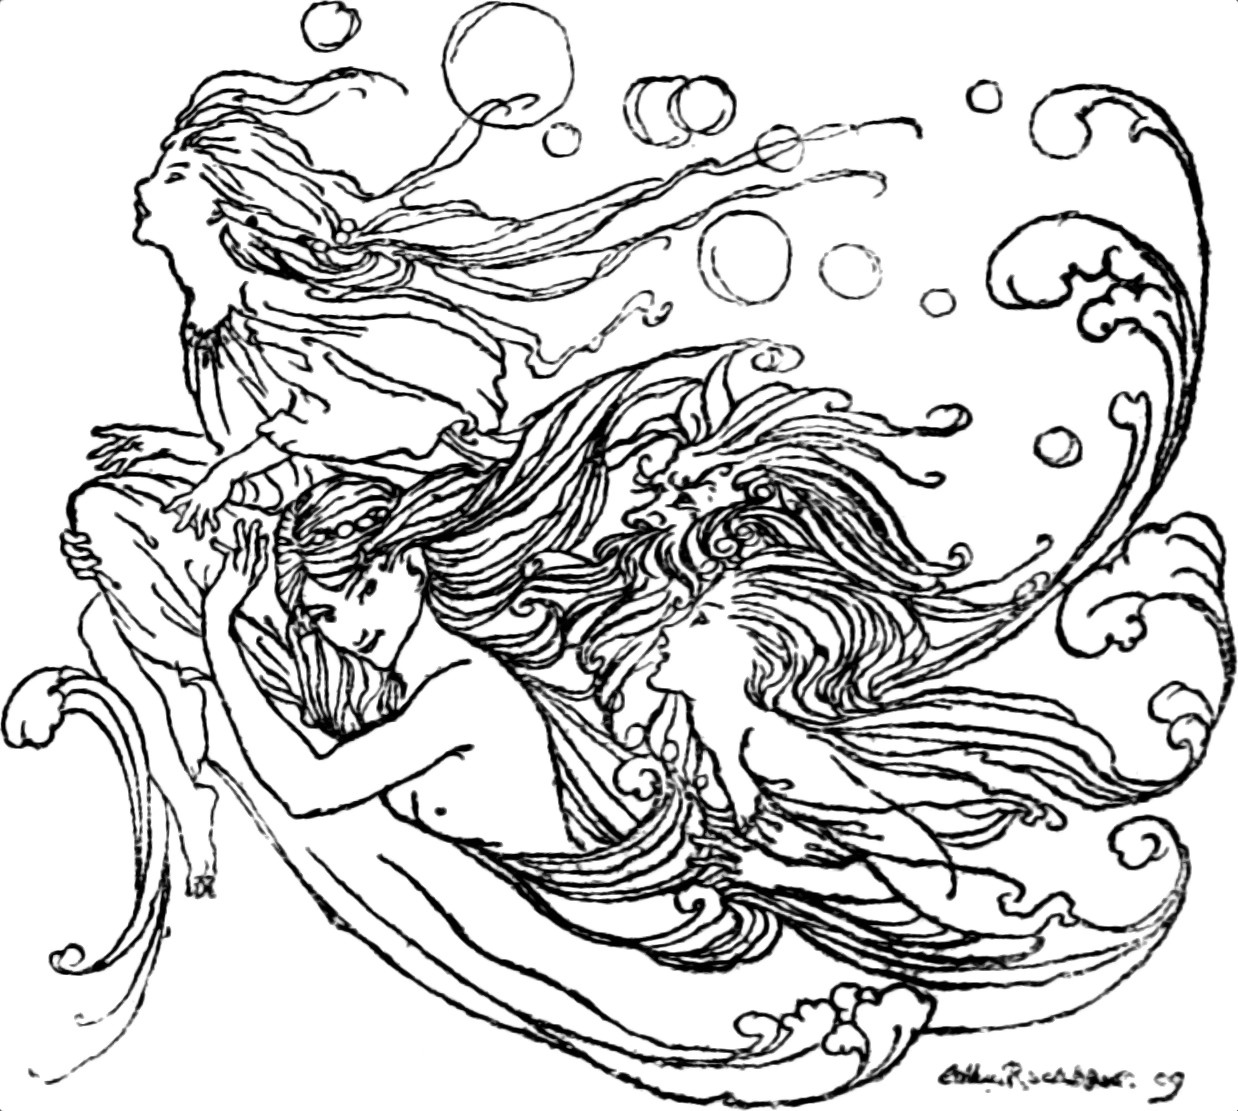
\includegraphics[width=.7\textwidth]{merwave}};
	\end{tikzpicture}
\end{letter}